\documentclass[11pt]{article}
\usepackage[margin=1cm]{geometry}
\usepackage[T1]{fontenc}
\pagenumbering{gobble}
\usepackage{graphicx}
\graphicspath{{img}}

\title{\vspace*{-1cm}Assembler, Extension and Group Reflection}
\date{\vspace*{-1cm}12 June 2021}

\begin{document}

\maketitle

\section{Introduction}
As the emulator and assembler are separate programs that can be tested and implemented independently, we have made a group decision to complete them in parallel. This report will omit the base implementation of the emulator, because it has already been mentioned in the checkpoint report. The workload was split as follows:
\begin{center}
	\begin{tabular}{ r | l }
		\textbf{Emulator} & \textbf{Assembler} \\
		Ioana \& Oliver & Bartłomiej \& Jordan
	\end{tabular}
\end{center}
\section{Assembler}
\subsection*{Workflow}
The development cycle for the assembler was very simmilar to that of the emulator:\\\\
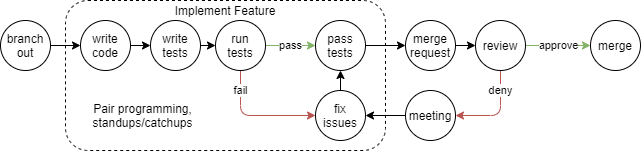
\includegraphics[width = \textwidth]{development cycle}
In addition, the workload of the assembler was split as follows:\\
\begin{center}
	\begin{tabular}{r|l}
		\textbf{Person Responsible} & \textbf{Feature} \\\
		Bartek & stddata library \\
		Jordan & main data flow \\
		Jordan & tokenizer \\
		Bartek & command processing \\
	\end{tabular}
\end{center}
\subsection*{StdData}
The stddata library, inspired by c++'s STL, has proved invaluable in the implementation of the assembler, although has not been utilized in the emulator. The library features the following structures, the interface of which mimics that of the stl library (with accommodations to the lack of some featues in c):
\begin{itemize}
\item Stack (unused) - an implementation of a vector-based stack
\item Queue (unused) - an implementation of a list-based queue
\item Deque (unused) - an implementation of a list-based deque
\item Vector - a resizable array with static time operations
\item VectorIterator - an iterator for looping over the elements of a vector
\item List - a linked list implementation
\item ListIterator - an iterator for looping over the elements of a list
\item Set - a hashset implementation with buckets implemented using linear probing
\item SetIterator - an iterator for looping over the elements of a set
\item Map - a hashmap implementation with buckets implemented using linear probing
\item MapIterator - an iterator for looping over the elements of a map
\item DecisionTree - a custom data structure simmilar to a trie working as a map with keys as sequences of items
\end{itemize}
The full documentation of this library (generated using doxygen) can be accessed under lib/stddata/doc/refman.pdf
\subsection*{Data Flow}
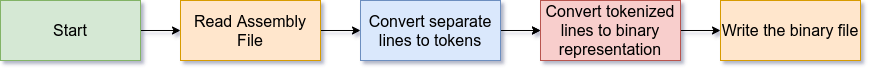
\includegraphics[scale=0.6]{assembler_dataflow}
\subsection*{Tokenization}
<A couple of lines explaining the tokenizer in assembler>
\subsection*{Command Generation}
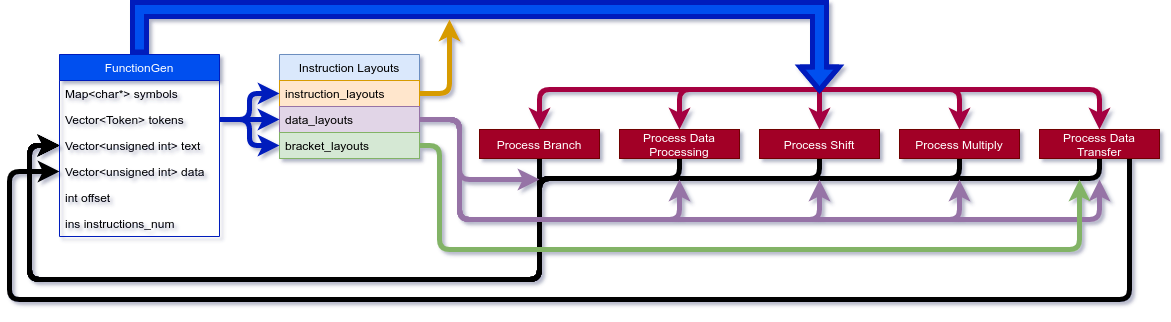
\includegraphics[width=\textwidth]{commandgen}
The command generation consist of 2 stages: processing function dispatch and data conversion to a binary representation. The processing function dispatch uses the sequence of the tokens and a decision tree to determine the appropriate function for the sequence. Then, now inside the processing funciton, it uses another decision tree to determine which fields inside the function need to be set according to which tokens. Since the fields can be set to some values before that step, this allows for highly flexible default values and a greatly reduced number of processing function (in a previous implementation without that feature the code was 3-4x longer). A simmilar decision tree is used for determining if a data transfer funciton is pre or post.
\subsection*{Testing}
<A couple of lines about the way we tested our code>
\section{Extension}
[2 pages]
For the extension we settled on adding enough support to the assembler and emulator to write a simple pong game in pure assembly, inspired by Atari's product with the same name from 1972. This decision was made based on many factors, including time left, team size, capabilities of the implementation at the moment of choosing and potential educational benefits for us.
\subsection*{Assembler}
The most extension was required by the assembler, having to add support for the data section, stack and subroutines. However, thanks to the foresight while writing the base implementation, this proved to be rather straigtforward.
\paragraph*{Data Section}
The data section added the capability to store data for our code, for example the images for our game or global variables. All of the contents of the data section are always stored after the instructions, i.e. the the text section.
\paragraph*{Assembler Directives} The support for assembler directives was required due to the data section and the need to collaborate on the code. After some research, we settled on supporting the following:
\begin{center}
	\begin{tabular}{r|l}
		\textbf{Directive} & \textbf{Purpose} \\
		.data & Signifies the start of the data section \\
		.text & Signifies the start of the text section \\
		.long <expression> & Places a 32-bit integer in the data section \\
		.set <label> <constant> & Sets the value of a label to a constant \\
		.include <filepath> & Pastes the contents of a file in its place
	\end{tabular}
\end{center}
The .include direcitve, altough not in the standard assembly, has allowed us to split our code into multiple files while removing a need to write a more elaborate solution, for example a linker.
\paragraph*{Additional Commands}
In order to support the stack and subroutines, the following extensions to the available commands were added:
\begin{center}
	\begin{tabular}{r|l}
		\textbf{Pattern} & \textbf{Explanation} \\
		bln (bl) <expression> & same as branch, but before branching places \\
		                      & the contents of r15(PC) into r14(LR) \\
		<ldr/str> Rn, [Rd, <operand>]! & same as pre data transfer instruction, \\
		                               & but places the new value of the address into Rd \\
		<instr><cond> ... & every instruction can now have a condition code
	\end{tabular}
\end{center}
along with the following aliases for the ease of use
\begin{center}
	\begin{tabular}{r|l}
		\textbf{Alias} & \textbf{Expanded form} \\
		ret<cond> & mov<cond> r15, r14\\
		push<cond> rn & str<cond> rn, [r13, \#-4]!\\
		pop<cond> rn & ldr<cond> rn, [r13] \#4\\
		hlt<cond> & andeq r0, r0, r0
	\end{tabular}
\end{center}
\paragraph*{Miscellaneous}
\begin{itemize}
\item Support for meaningful assembling errors
\item All constants can now be substituted for labels
\item All labels in expressions can now be offset by +/- value
\item :first8:label, :second8:label, ... allow for refering to bits of label separately (useful for loading a value of the label into a register)
\end{itemize}
\subsection*{Emulator}
<A couple of lines of introduction to the emulator extensions>
\paragraph*{Additional Commands}
<More detailed explanation of supporting the additional commands>
\paragraph*{Keystrokes}
<More detailed explanation of supporting the keystrokes>
\paragraph*{Display}
<More detailed explanation of supporting the display>
\subsection*{Pong}
\begin{center}
	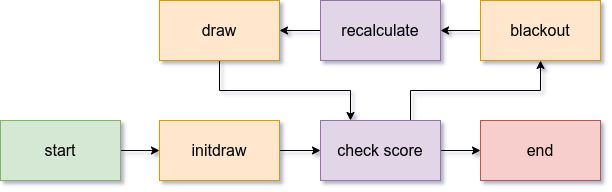
\includegraphics[scale=0.7]{pong}\\
\end{center}
\begin{tabular}{l|c|r}
	\textbf{Subroutine} & \textbf{Purpose} & \textbf{Assigned to}\\
	main & the main loop of the program & Jordan \& Oliver\\
	initdraw & draws the initial page of the pong game & Bartek \& Ioana\\
	blackout & removes the old instances of screen elements from the buffer & Bartek \& Ioana\\
	recalculate & performs the physics calculation and advances the time step & Jordan \& Oliver\\
	draw & draws the new components and updates the screen & Bartek \& Ioana\\
\end{tabular}
\section{Group Reflection}
\subsection*{Communication}
<A couple of lines on the quality of communication inside the group>
\subsection*{Individual Reflections}
\paragraph*{Jordan}
<Here go a couple of lines from Jordan on how he did in the project>
\paragraph*{Ioana}
<Here go a couple of lines from Ioana on how she did in the project>
\paragraph*{Oliver}
<Here go a couple of lines from Oliver on how he did in the project>
\paragraph*{Bartek}
<Here go a couple of lines from Bartek on how he did in the project>
\end{document}
